%% ----------------------------------------------------------------
%% Report.tex
%% ---------------------------------------------------------------- 
\documentclass{ecsreport2}      % Use the Report Style
\graphicspath{{./Figures/}}   % Location of your graphics files
\usepackage{natbib}            % Use Natbib style for the refs.
\hypersetup{colorlinks=false}   % Set to false for black/white printing
%% ----------------------------------------------------------------
%% Definitions.tex
%% ---------------------------------------------------------------- 
\newcommand{\BibTeX}{{\rm B\kern-.05em{\sc i\kern-.025em b}\kern-.08em T\kern-.1667em\lower.7ex\hbox{E}\kern-.125emX}}

%% People
\newcounter{address}
\setcounter{address}{1}
\renewcommand{\theaddress}{\textsuperscript{\fnsymbol{address}}}
\newcommand{\address}[1]{\refstepcounter{address}\theaddress#1\\}
\newcommand{\Name}[3]{\texorpdfstring{\href{mailto:#3}{#2}#1}{#2}\xspace}
\newcommand{\SteveRGunn}[1]{\Name{#1}{Steve R. Gunn}{S.R.Gunn@ecs.soton.ac.uk}}

%% Dingbats
\newcommand{\tick}{\ding{51}}
\newcommand{\cross}{\ding{55}}

%% Calculus
\newcommand{\pd}[2]{\ensuremath{\frac{\partial #1}{\partial #2}}\xspace}
\newcommand{\fd}[2]{\ensuremath{\frac{d #1}{d #2}}\xspace}
\newcommand{\dint}{\ensuremath{\int\!\!\!\int}\xspace}
\newcommand{\tint}{\ensuremath{\int\!\!\!\int\!\!\!\int}\xspace}

%% Math Sets
\newcommand{\Q}[1]{\ensuremath{\mathbb{#1}}\xspace}
\newcommand{\R}{\Q{R}}

%% Matrix, Vector
\newcommand{\V}[1]{\ensuremath{\boldsymbol{#1}}\xspace}
\newcommand{\M}[1]{\ensuremath{\boldsymbol{#1}}\xspace}
\newcommand{\0}{\V{0}}
\newcommand{\1}{\V{1}}
\newcommand{\I}{\M{I}}

%% Math Functions
\newcommand{\F}[1]{\ensuremath{\mathrm{#1}}\xspace}
\newcommand{\sgn}{\F{sgn}}
\newcommand{\tr}{\F{trace}}
\newcommand{\diag}{\F{diag}}

%% Math Names
\newcommand{\N}[1]{\ensuremath{\mathit{#1}}\xspace}

%% Data
\newcommand{\mc}[1]{\ensuremath{\mathcal{#1}}\xspace}
\newcommand{\Hyp}{\mc{H}}
\newcommand{\D}{\mc{D}}

%% Kernel
\newcommand{\K}{\M{K}}
\newcommand{\eins}{\texorpdfstring{\ensuremath{\epsilon}}{\textepsilon}-insensitive\xspace}
\newcommand{\e}{\ensuremath{\epsilon}\xspace}
\newcommand{\Bxi}{\ensuremath{\boldsymbol{\xi}}\xspace}
\newcommand{\Kanova}{\ensuremath{\mathit{K_{ANOVA}}}\xspace}
\newcommand{\Kspline}{\ensuremath{\mathit{K_{spline}}}\xspace}

%% Bayesian
\newcommand{\MP}{\ensuremath{\mathit{{\scriptscriptstyle \hspace{-1.5pt}M\hspace{-1.5pt}P}}}\xspace}
\newcommand{\ML}{\ensuremath{\mathit{{\scriptscriptstyle \hspace{-1.5pt}M\hspace{-1.5pt}L}}}\xspace}
\newcommand{\Qw}{\ensuremath{Q_{\w}(\w)}\xspace}
\newcommand{\Qa}{\ensuremath{Q_{\Ba}(\Ba)}\xspace}
\newcommand{\Qb}{\ensuremath{Q_{\beta}(\beta)}\xspace}
\newcommand{\wMPab}{\ensuremath{\w_{\MP|\bar {\Ba},\bar \beta}}\xspace}
\newcommand{\wMP}{\ensuremath{\w_{\MP}}\xspace}
\newcommand{\yMP}{\ensuremath{y_{\MP}}\xspace}
\newcommand{\BaMP}{\ensuremath{\Ba_{\hspace{1pt}\MP}}\xspace}
\newcommand{\aMP}{\ensuremath{\alpha_{\hspace{1pt}\MP}}\xspace}
\newcommand{\bMP}{\ensuremath{\beta_{\hspace{1pt}\MP}}\xspace}
\newcommand{\Sab}{\ensuremath{\M{\Sigma}_{\bar \Ba,\bar \beta}}\xspace}
\newcommand{\Ba}{\ensuremath{\boldsymbol{\alpha}}\xspace}
\newcommand{\Bb}{\ensuremath{\boldsymbol{\beta}}\xspace}
\newcommand{\Bm}{\ensuremath{\boldsymbol{\mu}}\xspace}
\newcommand{\BL}{\ensuremath{\boldsymbol{\Lambda}}\xspace}
\newcommand{\BPhi}{\ensuremath{\boldsymbol{\Phi}}\xspace}
\newcommand{\SMP}{\ensuremath{\M{\Sigma}_{\MP}}\xspace}

\newcommand{\Pa}{\ensuremath{P(\alpha|\mathcal{H})}\xspace}
\newcommand{\Pb}{\ensuremath{P(\beta|\mathcal{H})}\xspace}
\newcommand{\Pab}{\ensuremath{P(\alpha,\beta|\mathcal{H})}\xspace}
\newcommand{\Pw}{\ensuremath{P(\w|\mathcal{H})}\xspace}
\newcommand{\PD}{\ensuremath{P(\D|\mathcal{H})}\xspace}
\newcommand{\PwIa}{\ensuremath{P(\w|\alpha,\mathcal{H})}\xspace}
\newcommand{\PDIwb}{\ensuremath{P(\D|\w,\beta,\mathcal{H})}\xspace}
\newcommand{\PDwab}{\ensuremath{P(\D,\w,\alpha,\beta|\mathcal{H})}\xspace}
\newcommand{\PDIw}{\ensuremath{P(\D|\w,\mathcal{H})}\xspace}
\newcommand{\PwID}{\ensuremath{P(\w|\D,\mathcal{H})}\xspace}
\newcommand{\PwabID}{\ensuremath{P(\w,\alpha,\beta|\D,\mathcal{H})}\xspace}

\newcommand{\PanH}{\ensuremath{P(\alpha)}\xspace}
\newcommand{\PbnH}{\ensuremath{P(\beta)}\xspace}
\newcommand{\PabnH}{\ensuremath{P(\alpha,\beta)}\xspace}
\newcommand{\PwnH}{\ensuremath{P(\w)}\xspace}
\newcommand{\PDnH}{\ensuremath{P(\D)}\xspace}
\newcommand{\PwIanH}{\ensuremath{P(\w|\alpha)}\xspace}
\newcommand{\PDIwbnH}{\ensuremath{P(\D|\w,\beta)}\xspace}
\newcommand{\PDwabnH}{\ensuremath{P(\D,\w,\Ba,\beta)}\xspace}
\newcommand{\PDIwnH}{\ensuremath{P(\D|\w)}\xspace}
\newcommand{\PwIDnH}{\ensuremath{P(\w|\D)}\xspace}
\newcommand{\PwabIDnH}{\ensuremath{P(\w,\alpha,\beta|\D)}\xspace}

\newcommand{\PDwBab}{\ensuremath{P(\D,\w,\Ba,\beta|\mathcal{H})}\xspace}
\newcommand{\PwIBa}{\ensuremath{P(\w|\Ba,\mathcal{H})}\xspace}
\newcommand{\PBab}{\ensuremath{P(\Ba,\beta|\mathcal{H})}\xspace}
\newcommand{\PwBabID}{\ensuremath{P(\w,\Ba,\beta|\D,\mathcal{H})}\xspace}

\newcommand{\PBanH}{\ensuremath{P(\Ba)}\xspace}
\newcommand{\PwIBanH}{\ensuremath{P(\w|\Ba)}\xspace}

%% Snakes
\newcommand{\Esnake}{\ensuremath{\mathit{E_{snake}}}\xspace}
\newcommand{\Eimage}{\ensuremath{\mathit{E_{image}}}\xspace}
\newcommand{\Econt}{\ensuremath{\mathit{E_{cont}}}\xspace}
\newcommand{\Ecurv}{\ensuremath{\mathit{E_{curv}}}\xspace}
\newcommand{\Eint}{\ensuremath{\mathit{E_{int}}}\xspace}
\newcommand{\Eext}{\ensuremath{\mathit{E_{ext}}}\xspace}
\newcommand{\Eterm}{\ensuremath{\mathit{E_{term}}}\xspace}
\newcommand{\Eline}{\ensuremath{\mathit{E_{line}}}\xspace}
\newcommand{\Eedge}{\ensuremath{\mathit{E_{edge}}}\xspace}
\newcommand{\Econ}{\ensuremath{\mathit{E_{con}}}\xspace}
\newcommand{\Eangle}{\ensuremath{\mathit{E_{angle}}}\xspace}
\newcommand{\Elshape}{\ensuremath{\mathit{E_{lshape}}}\xspace}
\newcommand{\Eedgedir}{\ensuremath{\mathit{E_{edgedir}}}\xspace}
\newcommand{\Emodel}{\ensuremath{\mathit{E_{model}}}\xspace}
\newcommand{\wte}{\ensuremath{\mathit{w_{term}}}\xspace}
\newcommand{\wli}{\ensuremath{\mathit{w_{line}}}\xspace}
\newcommand{\wed}{\ensuremath{\mathit{w_{edge}}}\xspace}
\newcommand{\wco}{\ensuremath{\mathit{w_{con}}}\xspace}

%% Environments
\newcounter{alg}
\newenvironment{algorithm}[1]
{
    \stepcounter{alg}
    \begin{table}[htb]
    \centering
    \begin{tabular}[t]{ll}
    \hline&\\
    \multicolumn{2}{l}{\bf Algorithm \arabic{alg}: #1}\\&\\
} {
    &\\
    \hline
    \end{tabular}
    \end{table}
}
            % Include your abbreviations
%% ----------------------------------------------------------------
\begin{document}
\frontmatter
\title      {Modular Robot}
\authors    { {Nikhil Banerjee \\ John Charlesworth \\ Michael Hodgson \\ Max Lotz \\ Will Neep \\ Romel Torres}   }
\addresses  {\groupname\\\deptname\\\univname}
\date       {\today}
\subject    {Biologically-Inspired Robotics}
\keywords   {}
\maketitle
\begin{abstract}
This work is all about \dots
\end{abstract}
\tableofcontents
%\listoffigures
%\listoftables
%\lstlistoflistings
%\listofsymbols{ll}{$w$ & The weight vector}
%\acknowledgements{Thanks to no one.}
%\dedicatory{To \dots}
\mainmatter
%% ----------------------------------------------------------------
%% ----------------------------------------------------------------
%% Introduction.tex
%% ---------------------------------------------------------------- 
\chapter{Introduction} \label{Chapter:Introduction}
You probably found all the files from \cite{Gunn:2001:pdflatex}.
\tref{Table:tabex} illustrates the results of my work.
\begin{table}[!htb]
  \centering
  \begin{tabular}{cc}
  \toprule
  \textbf{Training Error} & \textbf{Testing Error}\\
  \midrule
  0 & $\infty$\\
  \bottomrule
  \end{tabular}
  \caption{The Results}
  \label{Table:tabex}
\end{table}

\fref{Figure:figex} shows why this is the case.
\begin{figure}[!htb]
  \centering
  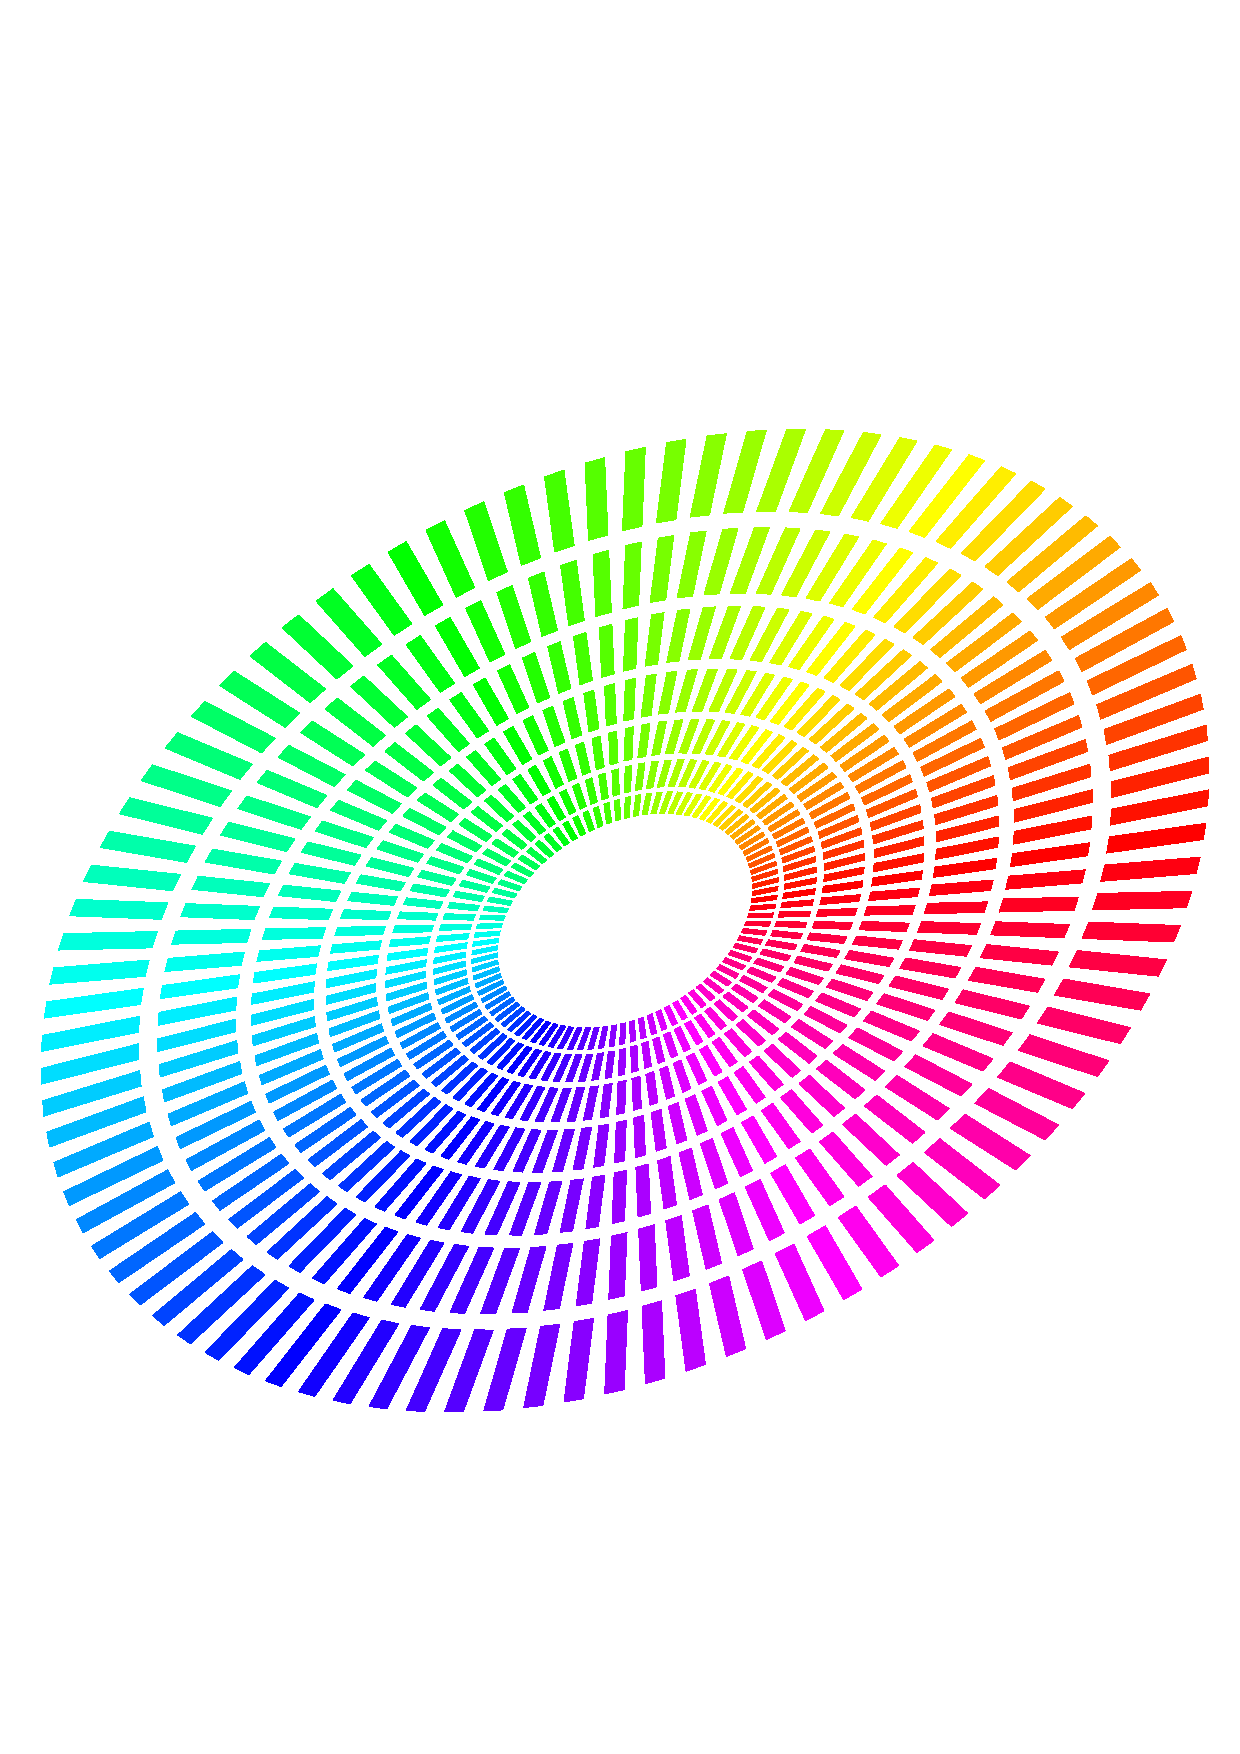
\includegraphics[width=8cm]{figure}
  \caption{A colourful picture.}
  \label{Figure:figex}
\end{figure}

This page shows you a subfigure example in \fref{Figure:figsubex}.
\begin{figure}[!htb]
  \centering
  \subfigure[The left caption]{
    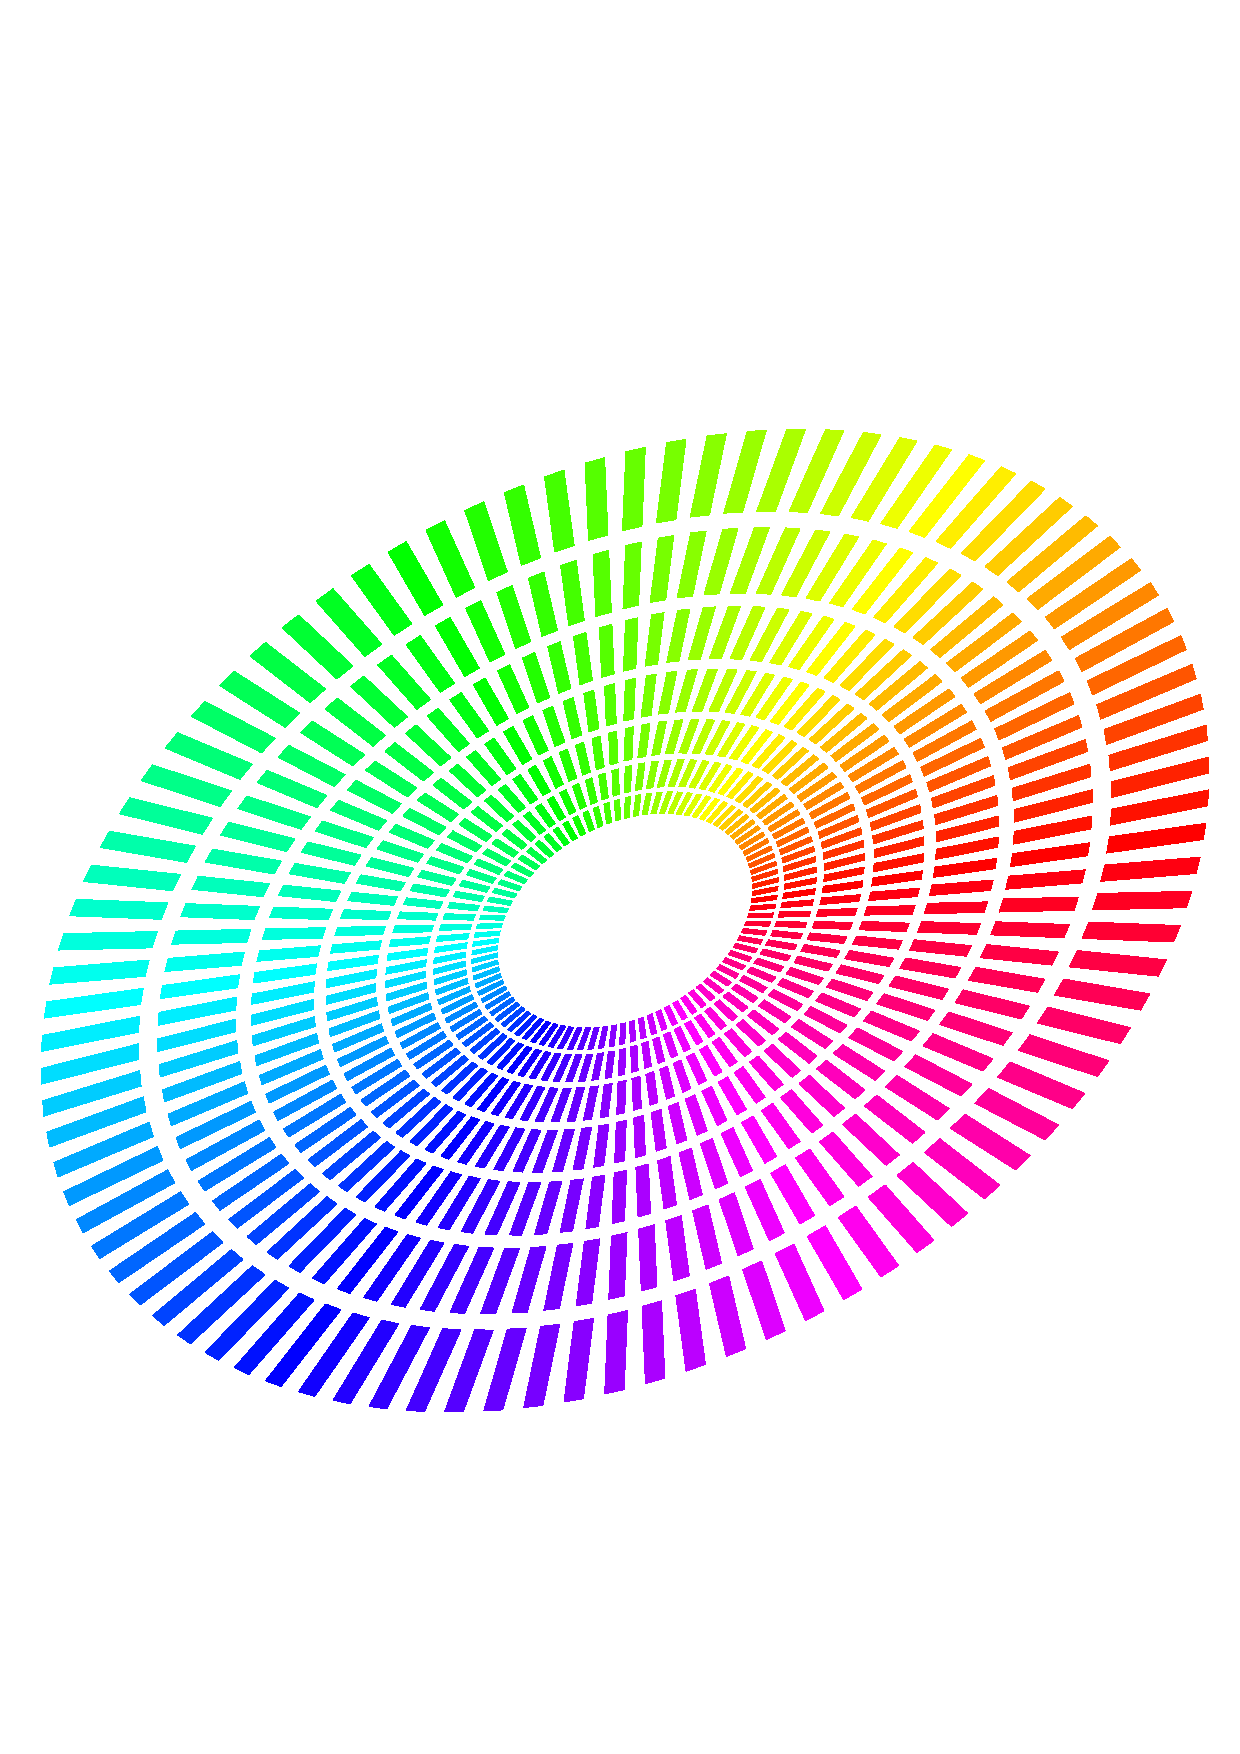
\includegraphics[width=4.2cm]{figure}
    \label{Figure:figsubex:left}
  }
  \subfigure[The right caption]{
    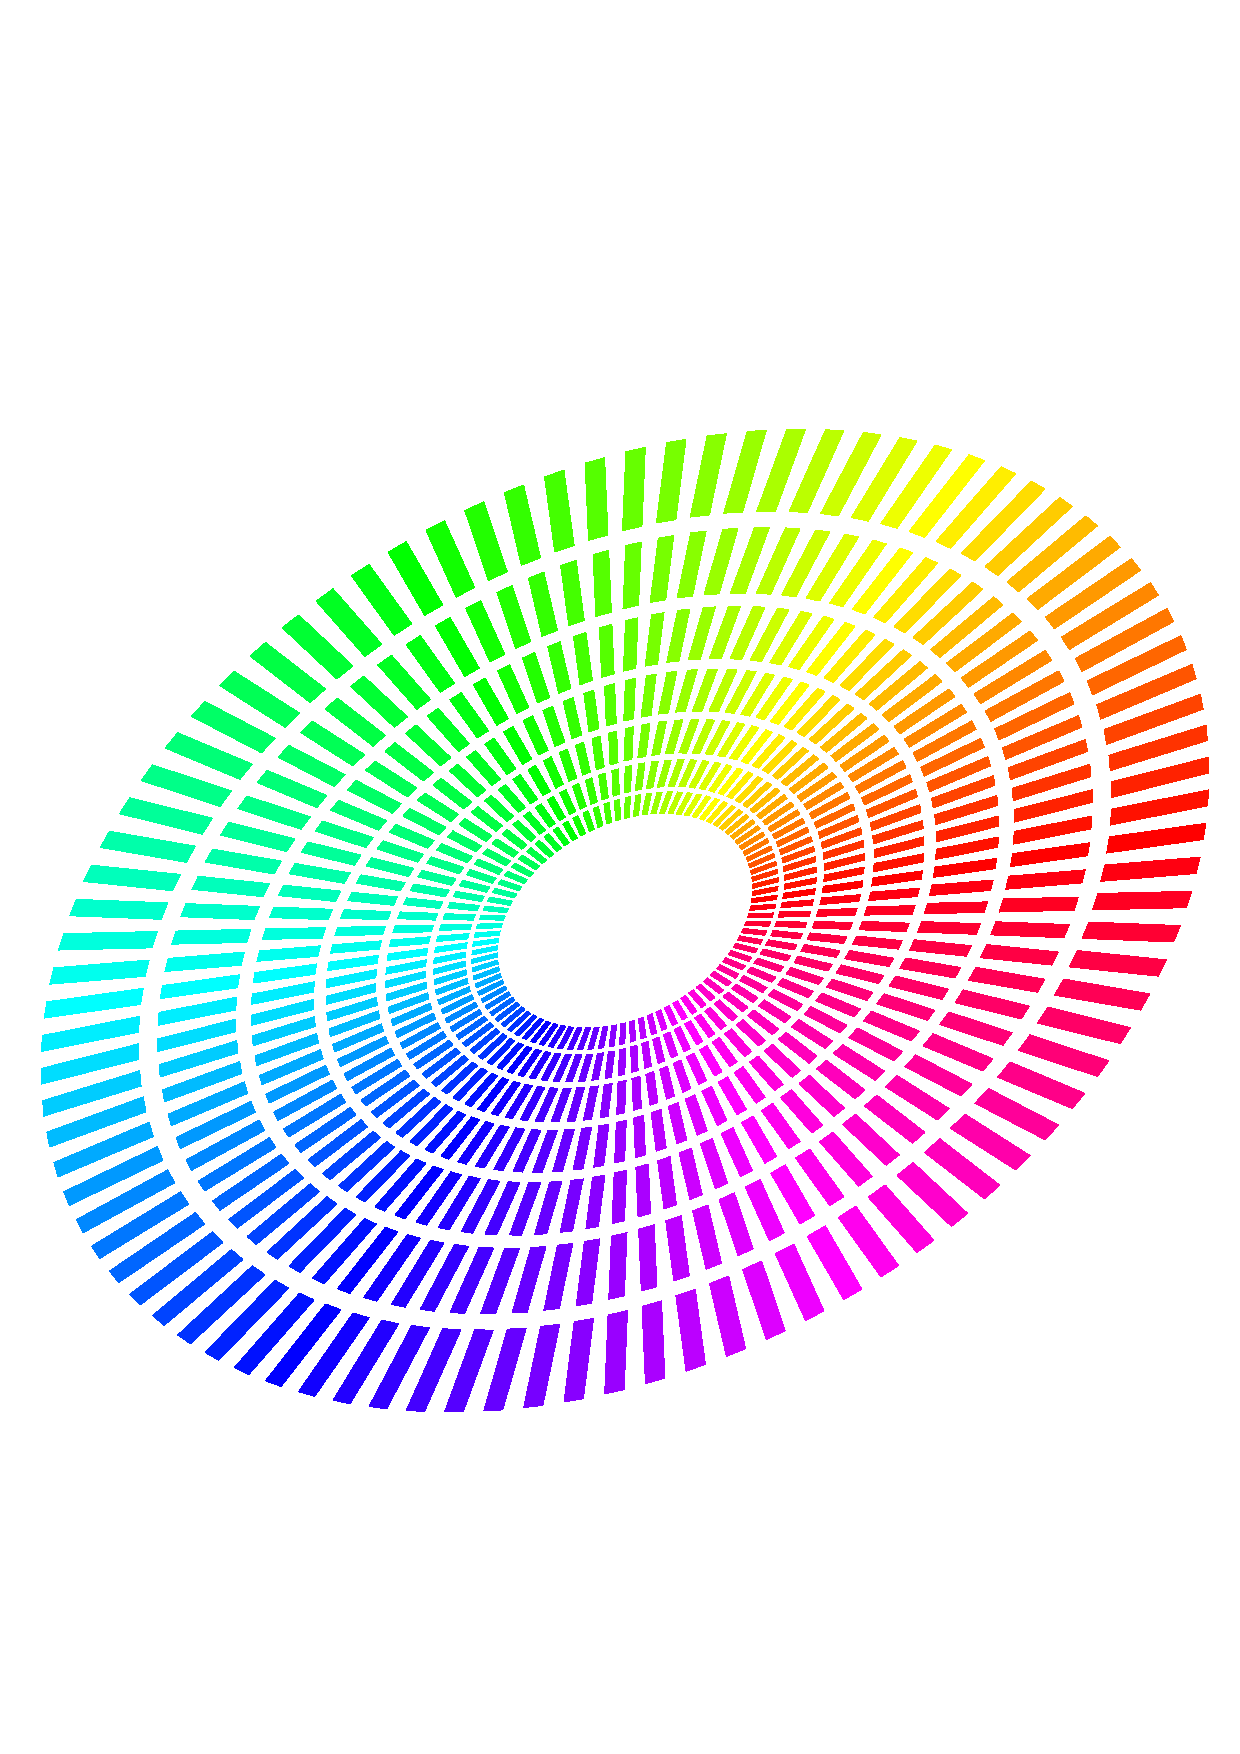
\includegraphics[width=4.2cm]{figure}
    \label{Figure:figsubex:right}
  }
  \caption{A doubly colourful picture.}
  \label{Figure:figsubex}
\end{figure}

%% ----------------------------------------------------------------
%% SystemOverview.tex
%% ---------------------------------------------------------------- 
\chapter{System Overview} \label{Chapter:SystemOverview}

an overview of the system \dots
%% ----------------------------------------------------------------
%% ElectroMechDesign.tex
%% ---------------------------------------------------------------- 
\chapter{Electromechanical Design} \label{Chapter:ElectroMechDesign}

\section{Servo}
Servos \dots

\section{Chassis}
Chassis \dots

\section{Prototyping}
Prototyping \dots

\section{Subsections}
Subsections \dots

\section{Summary etc}
Summary \dots
%% ----------------------------------------------------------------
%% ModuleElecDesign.tex
%% ---------------------------------------------------------------- 
\chapter{Module Electronics Design} \label{Chapter:ModuleElecDesign}

\section{Overview}
Overview \dots

\section{Communication}

\subsection{Why do we need it and what do we need Spec  m}

\subsection{Communications Overview m}

\subsection{Physical Layer m}

\subsection{Neighbor to Neighbor Packet Layer m}

\subsection{Network Layer}

\begin{figure}[htb]
\centering
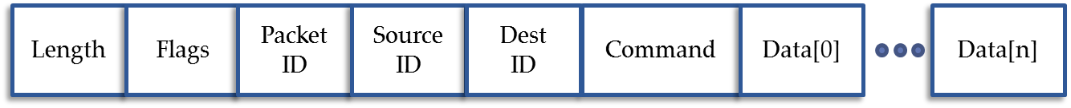
\includegraphics[width=0.8\textwidth]{images/network_packet.png}
\caption{Network Packet}
\label{fig:network_packet}
\end{figure}


\subsection{Application Layer - r}

\subsection{Prototyping and Implementation - r}

%%------------------------------------------------------------------
\section{Sensors}
%%------------------------------------------------------------------



%%------------------------------------------------------------------
\section{PCB Design}
%%------------------------------------------------------------------
\subsection{Advantages of PCB Design}
PCB circuit design is more compact and reliable than breadboard or stripboard based circuit. It also allows for the use of surface mount type components which both allows for further compactness and increases the range of available components that may be used.
Components used in the final circuit design were SOIC type surface mount components as these are small enough to allow for the proper compactness of the circuit, but can be soldered by hand. This increased the speed at which they could be constructed.

\subsection{Constraints}
The PCB was designed to be compatible with the Spirit Circuits Go Naked free prototyping service. This is a service whereby one copy of a PCB design is constructed for free, this allows a design to be refined before committing it to a production run. The constraints in place on this service are that the design can only include top and bottom copper layers and a drilling pattern.

\tref{Table:constraints} shows the minimum widths and distances for PCB construction with Spirit Circuits.
\begin{table}[!htb]
	\centering
	\begin{tabular}{cc}
	\toprule
	\textbf{Feature} & \textbf{Constraint}\\
	\midrule
	Minimum Track Width & 0.15mm (6mil) \\
	Minimum copper-copper spacing & 0.15mm (6mil) \\
	Minimum hole diameter & 0.3mm (12mil) \\
	\bottomrule
	\end{tabular}
	\caption{The Physical Design Constraints}
	\label{Table:constraints}
\end{table}

Other constraints on the design of the PCB come from the size of the physical chassis in which the circuit has to fit. The physical chassis size is based around the two servos; the space available for the circuit was measured as 120mm x 35mm.

\subsection{Design}
The circuit was designed, as part of the earlier work on the communication between modules, in cadence's OrCad software and the design of the PCB was done in National Instruments Utiliboard. Unfortunately it was not possible to copy the circuit across directly from one software to the other nor was it possible to copy the circuit into cadence's PCB design software as an intermediary software was not installed on the computers used. Because of this the circuit had to be copied across manually.

The components were first placed, including headers, and then arranged so that components are close to the headers associated with them but still have enough room around them to route copper properly. Components were then wired together as per the circuit diagram. As many of the unused pins as possible were broken out from the microcontroller.

\begin{figure}[!htb]
  	\centering
  	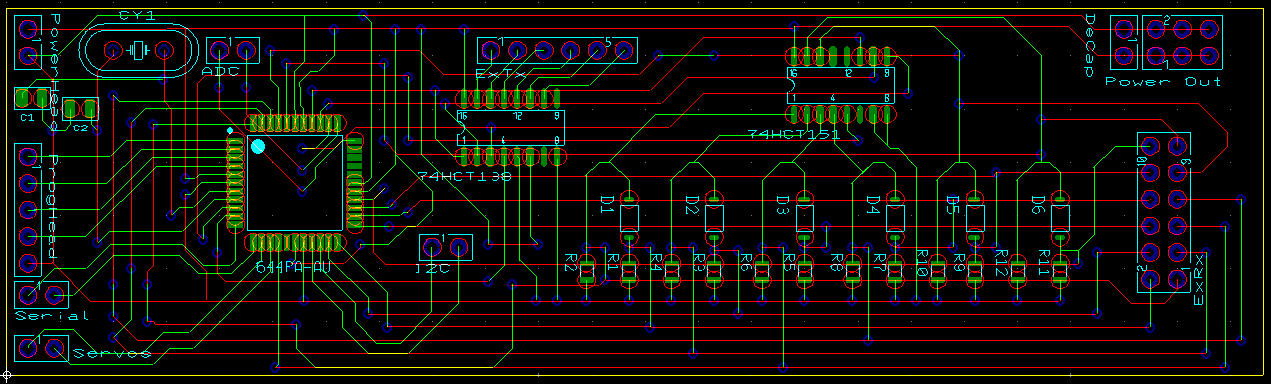
\includegraphics[width=\textwidth]{Figures/MainPCBDesign.png}
  	\caption{The Design for the Main Board}
 	\label{Figure:MainPCBDesign}
\end{figure}

In order to maximise the efficiency of the design routing has been mostly done so the horizontal wiring is on the bottom copper layer and vertical wiring is on the top copper layer and connections between these to are done with vias. At points this wiring scheme is impossible; for instance the microcontroller has both horizontal and vertical connections on the top copper layer.

Many of the sensors considered for use with the robot are only available in surface mount packages so in order to interface with them another PCB had to be designed, the particular packages of the sensors mean that they had to be soldered using solder paste and an oven. Some of the pin layouts for the sensors were non-standard so had to be manually constructed from measurements in the datasheets for use on the PCB.

\begin{figure}[!htb]
  	\centering
  	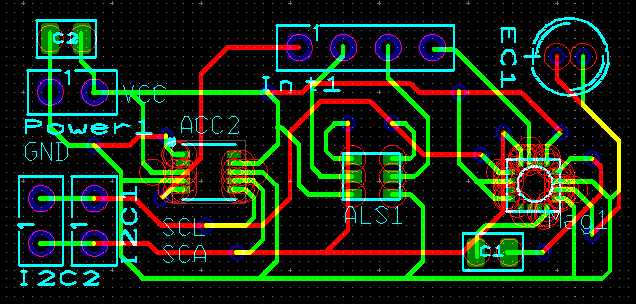
\includegraphics[width=0.5\textwidth]{Figures/SensorPCBDesign.png}
  	\caption{The Design for the Sensor Board}
 	\label{Figure:SensorPCBDesign}
\end{figure}

The sensor board was made separate from the main board in order to keep the main board design as general as possible. At 15mm x 36mm the sensor board was designed to fit into the chassis in either orientation for maximum versatility.

As further copies of the main board were needed for our system (it having been verified as working correctly) as well as the sensor board these were taken and panelised onto a standard eurocard sized board and send of again for another free prototype.


%%------------------------------------------------------------------
\section{Summary etc}
%%------------------------------------------------------------------
Summary \dots


%% ----------------------------------------------------------------
%% Simulation.tex
%% ---------------------------------------------------------------- 
\chapter{Simulation} \label{Chapter:Simulation}

\section{Overview}
Overview \dots

\section{Modelling}
Modelling \dots

\section{Movement}
Shake it \dots

\section{Communication}
Communication \dots

\section{Gaits}
Gaits \dots

\section{Summary etc}
Summary \dots
%% ----------------------------------------------------------------
%% Results.tex
%% ---------------------------------------------------------------- 
\chapter{Results} \label{Chapter:Results}


\include{Projectmanagement}
%% ----------------------------------------------------------------
%% Conclusions.tex
%% ---------------------------------------------------------------- 
\chapter{Conclusions} \label{Chapter: Conclusions}
It works.

%% ----------------------------------------------------------------
%% FurtherWork.tex
%% ---------------------------------------------------------------- 
\chapter{Further Work} \label{Chapter:FurtherWork}


\appendix
%% ----------------------------------------------------------------
%% AppendixA.tex
%% ---------------------------------------------------------------- 
\chapter{Stuff} \label{Chapter:Stuff}
The following gets in the way of the text....

%% ----------------------------------------------------------------
%% AppendixB.tex
%% ---------------------------------------------------------------- 
\chapter{Minutes} \label{Chapter:Minutes}
around 60 seconds \dots

%% ----------------------------------------------------------------
%% AppendixC.tex
%% ---------------------------------------------------------------- 
\chapter{Budget} \label{Chapter:Budget}
Spending of monies \dots

%% ----------------------------------------------------------------
%% AppendixD.tex
%% ---------------------------------------------------------------- 
\chapter{Gantt Charts} \label{Chapter:GanttCharts}
When it all happened \dots

\backmatter
\bibliographystyle{ecs}
\bibliography{ECS}
\end{document}
%% ----------------------------------------------------------------
